\subsection{Verifica della documentazione}
	Per la verifica della documentazione si utilizza la tecnica del \glock{walkthrough} revisionando i documenti per intero e la tecnica di \glock{inspection}. 

\subsubsection{Calcolo leggibilità e controllo ortografia dei documenti}
	Per verificare quanto sono leggibili i documenti redatti si utilizza l'\glock{indice di gulpease} ed è stato effettuato un controllo di ortografia, di seguito la tabella contenente i risultati ottenuti durante il periodo di analisi dei requisiti:

\begin{table} [h!]
	\rowcolors{2}{gray!25}{gray!6}
	\begin{center}
		\begin{tabular} { c c c c}
			\rowcolor{lightgray}
			\textbf{Documento}&\textbf{Errori ortografici}&\textbf{Indice di gulpease}&\textbf{Esito}\\
			\dext{Piano di progetto v1.0.0}		&0  & 59  &Superato\\
			\dext{Norme di progetto v1.0.0} 	&0	& 64  &Superato\\
			\dext{Studio di fattibilità v1.0.0}	&0	& 57  &Superato\\
			\dext{Glossario v1.0.0}				&0	& 47  &Superato\\
			\dext{Piano di qualifica v1.0.0}	&0	& 48  &Superato\\
			\dext{Media verbali v1.0.0}			&0	& 68  &Superato\\
			\dext{Analisi dei requisiti v1.0.0}	&0	& 72  &Superato\\
		\end{tabular}
	\end{center}
	\caption{Esiti verifiche automatizzate - Revisione Analisi dei requisiti}
\end{table}

Con il seguente grafico illustriamo l'andamento dell'indice di gulpease ad ogni revisione effettuata:

\begin{figure}[H]
	\centering
	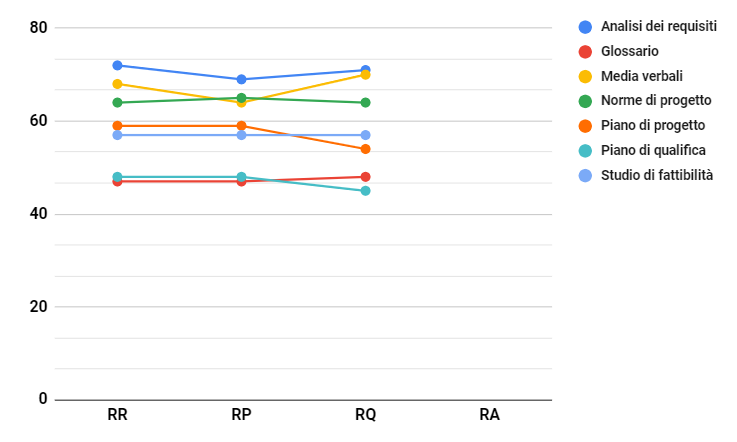
\includegraphics[width=13cm]{images/gulpease.png}
	\caption{Indice di gulpease per revisione}
\end{figure}

\subsection{}